\documentclass[10pt]{report}

\usepackage[utf8]{inputenc}
\usepackage[french]{babel}
\usepackage{amsmath}
\usepackage{amsfonts}
\usepackage{amssymb}
\usepackage{graphicx}
\usepackage{parskip}

\begin{document}

\title{Rapport - Devoir 1}
\date{Octobre 2010}
\author{Vincent Foley-Bourgon (FOLV08078309) \and
  Eric Thivierge (THIE09016601)}

\maketitle

\section{Fonctionnement général du programme}

Le programme effectue, dans l'ordre, les opérations suivantes:

\begin{enumerate}
  \item Lecture d'une chaîne.
  \item Détection des erreurs de syntaxe.
  \item Construction d'un arbre syntaxique abstrait.
  \item Évaluation du résultat.
  \item Détection des erreurs de sémantique.
  \item Affichage.
  \item Retour à l'étape 1.
\end{enumerate}


\subsection{Lecture d'une chaîne}

La lecture de la chaîne entrée par l'utilisateur se fait caractère par
caractère.  Le programme effectue en parallèle la lecture, la détection
d'erreurs de syntaxe et la construction de l'ASA (décrits ci-dessous).

\subsection{Détection des erreurs de syntaxe}

Aussitôt qu'une erreur de syntaxe est détectée, la fonction GenerateAST vide
le tampon d'entrée, libére les structures de données temporaires et retourne
un code d'erreur.

\subsection{Construction d'un arbre syntaxique abstrait}

Après la lecture d'un nombre, le programme l'ajoute à une pile d'expressions
(une structure définie plus tard).  Après avoir lu un opérateur, le programme
combine l'opérateur avec les deux dernières expressions sur la pile, et ajoute
cette nouvelle expression sur la pile.

\subsection{Évaluation du résultat}

Le programme évalue récursivement chaque noeud de l'ASA à partir de la
racine. Un noeud externe est évalué à la valeur numérique qu'il contient. Un
noeud interne contient un opérateur et le programme évalue ce noeud en
appliquant cette opération aux valeurs des sous-expressions gauches et
droites.

\subsection{Détection des erreurs de sémantque}

Le programme active un code d'erreur pendant l'évaluation du résultat s'il
détècte une division par zéro.


\subsection{Affichage}

Le programme affiche la représentation de l'expression syntaxiquement et
sémentiquement valide dans les syntaxes Scheme, C et Postscript suivi du
résultat de l'évaluation de l'expression.  Autrement, le programme affiche un
message d'erreur indiquant la nature du problème de l'expression.


\section{Représentation des ASAs}

Le programme utilise un arbre binaire pour représenter l'arbre de syntaxe
abstraite. Les noeuds internes de l'arbre représentent des opérateurs et les
feuilles des nombres.

\[
\text{Expression} =
\left\{
\begin{tabular}{l}
  \text{Nombre} \\
  \text{(Opérateur, Expression, Expression)}
\end{tabular}
\right.
\]

Dans l'implémentation en C, cette structure est représenté par le type
suivant:

\begin{verbatim}
struct Expr {
    enum { operand, expr } type;
    union {
        Number number;
        struct BinaryOperator {
            enum Operator operator;
            struct Expr *left;
            struct Expr *right;
        } expression;
    } _;
};
\end{verbatim}

L'union stocke soit un nombre, soit une expression binaire comportant un
opérateur et deux sous-expressions.  Le champ \emph{type} indique quel champ
de l'union est présentement stocké en mémoire.


\newpage

\section{Analyse syntaxique}

La fonction \emph{GenerateAST} prend en charge les tâches de lecture des
caractères, de création de l'ASA et de détection des erreurs.

\textbf{Tous les états:} un caractère est lu.  S'il s'agit de EOF, le
programme retourne le code \emph{ec\_eof}.  Si le caractère est invalide, le
programme vide le tampon d'entrée et retourne le code
\emph{ec\_invalid\_symbol}.

\textbf{st\_normal:} si le caractère lu est un chiffre, le programme met sa
valeur numérique dans la variable \emph{number} et passe à l'état
\emph{st\_number} pour lire un nombre.  Si le caractère est un opérateur, le
programme tente de dépiler deux expressions de la pile et de les combiner avec
l'opérateur en une nouvelle expression et l'état passe à \emph{st\_operator}.
S'il n'y a pas suffisament d'expressions sur la pile, le programme vide le
tampon d'entrée, libère -- s'il y a lieu -- les expressions temporairement
allouées et retourne le code \emph{ec\_invalid\_syntax}.

\textbf{st\_number:} si le caractère lu est un nombre, le programme met à jour
la variable \emph{number} en multipliant sa valeur par 10 et y ajout la valeur
numérique du caractère lu.  Si le caractère lu est un opérateur, c'est une
erreur de syntaxe; le programme vide le tampon d'entrée et retourne le code
\emph{ec\_invalid\_syntax}.  Si le caractère est un espace, le programme
construit une nouvelle expression à partir de \emph{number} et ajoute cette
expression à la pile.

\textbf{st\_operator:} lorsqu'on est dans l'état \emph{st\_operator}, c'est
que le caractère précédent était un opérateur.  Si le programme lit un chiffre
ou un autre opérateur, la syntaxe de l'expression est invalide.  Le programme
vide alors le tampon d'entrée et retourne le code \emph{ec\_invalid\_syntax}.
Si le caractère lu est un espace, on revient dans l'état \emph{st\_normal}.

\textbf{Après la boucle:} s'il reste un seul élément sur la pile, le programme
le met dans le paramètre \emph{out} et retourne \emph{ec\_ok}, sinon il
retourne \emph{ec\_invalid\_syntax}.  S'il n'y avait pas d'élément sur la
pile, le programme retourne \emph{ec\_empty\_expression}.

La figure suivante résume le fonctionnement de la fonction \emph{GenerateAST}:

\begin{center}
  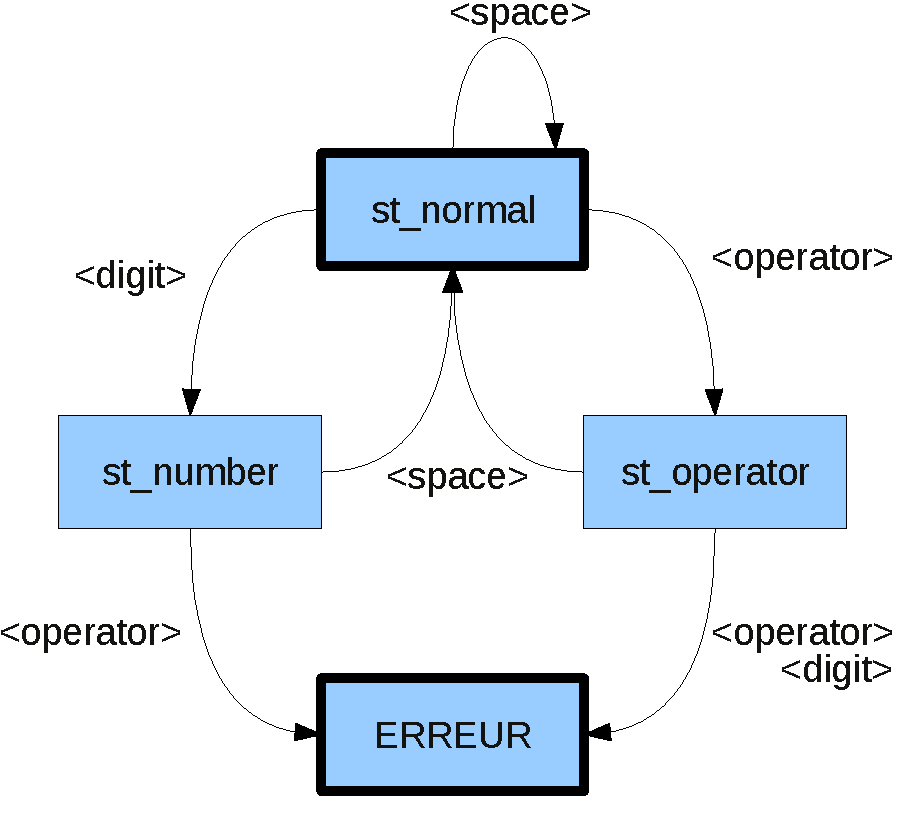
\includegraphics[scale=0.33]{statemachine}
\end{center}


\newpage

\section{Minmisation des parenthèses en syntaxe C}
À partir de la racine, le programme applique les règles suivantes à chaque noeud de
l'ASA:

Si le noeud visité contient un opérateur d'addition ou de soustraction,
les sous-expressions de gauche et de droite ne sont pas parentèsées.

Si le noeud visité contient un opérateur de multiplication ou de division
alors le programme traite les sous-expressions de gauche et de droite de la
façon suivante:

\textbf{Sous-expression de gauche}

Parenthèser la sous-expression de gauche si elle contient un opérateur d'addition ou de soustraction.

\textbf{Sous-expression de droite}

Parenthèser la sous-expression de droite dans les cas suivants:

\begin{itemize}
\item la sous-expression contient un opérateur d'addition ou de soustraction
\item le noeud visité contient un opérateur de multiplication et la sous-expression un opérateur de division
\item le noeud visité contient un opérateur de division et la sous-expression un opérateur de multiplication
\end{itemize}

\section{Traitement des erreurs}
Le programme traite deux catégories d'erreur, les erreurs système et
d'application.

\textbf{Erreurs système}

Le programme traite le cas où un appel à \emph{malloc} échoue. Si cela se
produit, le programme appelle la procédure \emph{OUT\_OF\_MEMORY()}, qui affiche un message
d'erreur et quitte proprement l'application en faisant un \emph{abort()}.

\textbf{Erreurs d'application}

L'énumération \emph{ErrorCode} contient tous les codes d'erreur utilisés dans
le programme. Le programme utilise les codes d'erreurs suivantes:

\begin{itemize}
\item ec\_ok: indique que l'opération a terminé sans erreur.
\item ec\_invalid\_syntax: indique une erreur de syntaxe dans l'expression
lue.
\item ec\_empty\_expression: indique qu'il n'y a pas d'expression sur la pile. 
\item ec\_div\_zero: indique que l'expression lue contient une division par
zéro.
\item ec\_invalid\_symbol: indique que l'expression lue contient un symbole
non valide.
\item ec\_eof: indique qu'il n'y a plus d'expression à traiter.
\end{itemize}


\section{Récupération de la mémoire}

La récupération de la mémoire est faite par des fonctions
``destructeurs'' qui vont faire la récupération de leurs éléments
internes.

\textbf{StackFree:} cette fonction parcourt tous les noeuds d'une pile
et appelle \emph{NodeFree} sur ces noeuds.  Lorsque tous les noeuds
ont été récupéré, \emph{StackFree} appelle \emph{free} sur le pointeur
de la pile qui lui a été passé.

\textbf{NodeFree:} cette fonction appelle \emph{ExprFree} sur sa
valeur et appelle ensuite \emph{free} sur le pointeur du noeud qui lui
a été passé.

\textbf{ExprFree:} cette fonction appelle (récursivement)
\emph{ExprFree} sur ses membres de gauche et de droite et appelle
ensuite \emph{free} sur le pointeur de l'expression qui lui a été
passé.

\textbf{StackPop:} dans la fonction \emph{StackPop}, le destructeur
\emph{NodeFree} n'est pas appelé, car il détruirait également
l'expression qu'on veut retourner.  C'est pourquoi il y a un appel
manuel à la fonction \emph{free}.  C'est le seul endroit dans le
programme où une donnée n'est pas détruite par un destructeur.


\end{document}
